\chapter{Bedrijf}
\label{ch:bedrijf}
Dit hoofdstuk biedt informatie over het bedrijf waarbij het onderzoek is uitgevoerd. Hiernaast geeft het inzicht in welke afdeling van het bedrijf het onderzoek gedaan is. 

\section{\&ranj}
\&ranj is een internationaal bedrijf dat al sinds 1999 serious game oplossingen realiseert. Dit zijn spellen waarbij de speler spelenderwijs getraind wordt. Een voorbeeld hiervan is de serious game ‘Mission Zhobia – Winning the Peace’\footnote{\url{https://www.missionzhobia.org/}} waarin de speler getraind wordt in peace building. Het bedrijf heeft te maken met klanten in totaal verschillende vakgebieden. Hierdoor is het domein van de onderwerpen erg breed.

\&ranj wilt mensen helpen ontwikkelen op een effectieve en efficiënte manier. Met behulp van ‘serious games’ wilt het bedrijf voor de gebruiker een ervaring creëren waarin hij of zij kennis opdoet om in het echte leven uitdagingen aan te gaan en leert problemen te tackelen. Volgens \&ranj is de beste manier van leren het leren door te doen.

\section{Visie}
Met serious games bereikt \&ranj op spelenderwijze gedragsverandering toepassen en om zo een betere toekomst te bouwen:

\begin{quote} 
    \centering
    \large
    \textit{
        “Together we build a brighter future”
    }
\end{quote}

\section{Afdelingen}
Het bedrijf verdeelt zich over drie verschillende afdelingen met ieder zijn eigen specialiteit:
\begin{itemize}
    \item Gamification; gefocust op: “consultancy”, “leuk maken van minder leuke taken/ werk”, “fysiek”.
    \item Playground; gefocust op: “experimentatie” en “ervaringen”.
    \item Corporate Learning; gefocust op: “soft skills”, “volwassen organisaties”, “bewezen oplossingen” en “efficiëntie”.
\end{itemize}
Dit onderzoek vindt plaats in de ‘coperate learning’ afdeling.

\section{Corporate learning}
De corporate learning afdeling van \&ranj realiseert oplossingen voor “volwassen” bedrijven die soft skills willen bevorderen. Bij deze afdeling ligt de nadruk op efficiëntie en het gebruikt van oplossingen waarvan het bedrijf weet dat ze werken. Meestal zijn deze oplossingen narrative games, spellen waarin op verhalende wijze kennis wordt bijgebracht. 

Het ontwikkelen van een narrative game is een heel proces, maar dit onderzoek zal zich alleen focussen op de ontwikkelingsfase. In deze fase werkt het team samen om het product te realiseren.

\begin{wrapfigure}{r}{0.45\textwidth}
    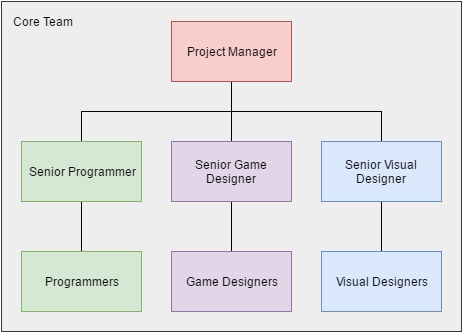
\includegraphics[width=0.43\textwidth]{CoreTeam}
    \caption{Anatomie van een core team bij \&ranj.}
    \label{fig:coreteam}
    \centering
\end{wrapfigure}

Een corporate learning development team bestaat meestal uit de volgende disciplines:

\begin{description}
    \item[Programmer] Is verantwoordelijk voor de technische implementatie van de serious game. 
    \item[Game designer] Is verantwoordelijk voor de mechanieken en het verhaal achter de game. Hij of zij probeert gedragsverandering toe te passen met de game als tool. Verder werken game designers nauw samen met de projectmanager om te zorgen dat de game aansluit bij de wensen van de klant.
    \item[Visual designer] Is verantwoordelijk voor de visuals binnen de game. Een visual designer wilt door middel van deze visuals meestal een gevoel bij de speler ontvlammen.
    \item[Projectmanager] Begeleid het ontwikkelproces en is regelmatig in contact met de klant. Hij of zij zorgt dat het project binnen het budget blijft en onderhandeld met de klant wanneer nodig. De projectmanager trekt aan de bel als het project niet aansluit bij de wensen van de klant en heeft veto op de keuzes binnen het project.    
\end{description}

